\chapter{Metodologia e Sviluppo}
\label{ch:metodologiasviluppo}

In questo capitolo verranno presentati la metodologia e lo sviluppo delle
soluzioni proposte nel capitolo \ref{sec:contributo} per l'ottimizzazione della
libreria \textit{CoopeRIS}. Verranno descritte le fasi di analisi, progettazione
ed implementazione, con particolare attenzione alle scelte effettuate e alle
motivazioni che hanno portato alla realizzazione delle stesse. Infine, sarà
presente una discussione sui vantaggi, svantaggi e limiti di ciascuna soluzione,
oltre che alle sfide affrontate durante lo sviluppo.

\section{Stato dell'arte della libreria \textit{CoopeRIS}}
\label{sec:libreria}

La libreria \textit{CoopeRIS} non è particolarmente complessa e rispecchia i
principi della programmazione ad oggetti. Tuttavia, presenta alcune criticità
nei metodi che implementa che ne limitano l'efficienza e la scalabilità, in particolare
nelle procedure di calcolo del \textit{guadagno} del segnale riflesso dalla RIS.
Questo sottocapitolo si propone di fornire una panoramica generale della libreria
in oggetto e delle sue funzionalità principali, oltre che la ricerca delle
possibili aree di ottimizzazione della stessa.

\subsection{Architettura e funzionamento}
\label{sec:architettura}

Il suo funzionamento è basato su un'architettura a classi in cui ogni istanza rappresenta
una RIS, i suoi metodi implementano le operazioni necessarie al fine di
calcolare le grandezze fisiche e geometriche utili alla simulazione, ed infine sfrutta
la libreria \textit{GSL}\cite{gnugsl} per la manipolazione di vettori e matrici,
reali e complesse. Le due procedure principali sono le seguenti:

\begin{itemize}
  \item \texttt{computePhases}: calcola le fasi dei singoli elementi dati gli angoli
    di incidenza, riflessione, trasmettitore e ricevitore salvando i risultati sulla
    matrice di configurazione della RIS denominata \texttt{coding}. Implementa le
    equazioni \ref{eq:phase-phi} e \ref{eq:phase-theta};

  \item \texttt{gain}: calcola il guadagno isotropico del segnale riflesso dalla
    RIS dati gli angoli di trasmettitore e del ricevitore, diretta derivazione
    dell'equazione \ref{eq:gain} e \ref{eq:power}.
\end{itemize}

In una esecuzione tipica, la prima fase prevede di calcolare gli sfasamenti di ogni
elemento radiante tramite la funzione \texttt{computePhases}, salvando la configurazione
sulla matrice denominata $coding$, ovvero lo stato degli elementi della RIS, per
poi calcolare il guadagno del segnale riflesso tramite il metodo \texttt{gain}.

\subsection{Identificazione dei colli di bottiglia e aree di ottimizzazione}
\label{sec:ottimizzazione}

Il metodo \texttt{computePhases} non è particolarmente soggetto a criticità in
quanto la sua complessità computazionale è lineare rispetto al numero di
elementi della RIS. Inoltre, dopo una prima profilazione, la procedura risulta già
essere sufficientemente veloce e ottimizzata. Il metodo \texttt{gain},
osservabile nel dettaglio nel listato \ref{lst:gain}, è invece più complesso e richiede
un numero molto maggiore di operazioni. La procedura di calcolo del guadagno è
infatti basata su un doppio ciclo \texttt{for} annidato, che scorre tutti gli
elementi della RIS e calcola il contributo di ciascuno di essi al guadagno
totale, per ogni possibile elemento sferico, come in equazione \ref{eq:gain} e
\ref{eq:power}. Questo comporta che il metodo \texttt{gain} scali
computazionalmente in maniera quadratica rispetto al numero di elementi della
RIS e alla scelta di discretizzazione dei possibili angoli $\phi$ e $\theta$ (aumentando
di conseguenza il numero di elementi sferici).

\vspace{1em}
\lstinputlisting[caption=Metodo \texttt{gain} della libreria \textit{CoopeRIS}, language=C++,
label=lst:gain]{listings/original-gain.cpp}
\vspace{1em}

Dopo una prima analisi statica del codice, si possono identificare quali parti
di esso corrispondano alle operazione matematiche descritte nelle equazioni
\ref{eq:power} e \ref{eq:gain}:

\begin{itemize}
  \item Le righe 18-19 sono i due cicli \texttt{for} annidati che scorrono tutti
    gli elementi della RIS, indicati dalle sommatorie in equazione \ref{eq:power};

  \item Le matrici $k\_du\_sin\_cos$ e $k\_du\_sin\_sin$ nelle righe 24-25 (che
    sono calcolate nella fase di inizializzazione della RIS in quanto statiche) corrispondono
    alla parte del termine $\Theta_{m,n}$ dipendente solamente dalla posizione del
    ricevitore, per ogni possibile angolo discreto $\phi$ e $\theta$. Queste sono
    successivamente moltiplicate rispettivamente per $n$ e $m$, ovvero la
    posizione dell'elemento RIS, per poi essere sommate, sia tra di loro, che con
    il corrispettivo termine $\Phi_{m,n}$ e \texttt{alpha}, ovvero la parte di $\Theta
    _{m,n}$ dipendente dalla posizione del trasmettitore. Questo ha lo scopo di
    calcolare il termine $\Phi_{m,n}+\Theta_{m,n}$ in equazione \ref{eq:power};

  \item Alle righe 35-36 è presente la moltiplicazione per $-j$ dei precedenti termini
    e l'applicazione della funzione esponenziale, come in equazione
    \ref{eq:power};

  \item A riga 38 si trova è la somma di $\textbf{P}_{\phi_{rx},\theta_{rx}}$ per
    elemento della RIS nella matrice \texttt{phase}, utile per il calcolo del guadagno
    totale $\texttt{p\_tot}$ utilizzato in equazione \ref{eq:gain};

  \item Le righe 59-61 corrispondono al calcolo del guadagno del segnale $\texttt
    {p\_tot}$ espresso da $\textbf{G}$ in equazione \ref{eq:gain}
\end{itemize}

Si può notare inoltre un layer di cache nelle righe 10-12 e 70, implementato in
quanto permette di evitare il ricalcolo di valori già calcolati in precedenza.

Considerando della Legge di Amdahl discussa nel capitolo \ref{sec:amdahl}, i due
cicli \texttt{for} rappresentano la porzione del codice ottimale per le
ottimizzazioni in oggetto in quanto sarà quella che meglio beneficerà della
parallelizzazione. Inoltre, questa specifica sezione è ulteriormente vantaggiosa
poiché tutte le iterazioni sono indipendenti tranne che per la somma finale
nella matrice \texttt{phase}, e per questo è stato il punto di partenza per la
progettazione delle soluzioni proposte.

\section{Implementazione delle soluzioni proposte}
\label{sec:implementazione}

Le soluzioni proposte per l'ottimizzazione del metodo \texttt{gain} sono basate
su due approcci differenti: la parallelizzazione tramite \textit{multi-threading}
e la parallelizzazione su GPU. Entrambe presentano piccole differenze, ma
condividono lo stesso obiettivo: ridurre il tempo di esecuzione nel calcolo della
matrice \texttt{phase} nei \texttt{for} annidati a righe 18-19 del codice \ref{lst:gain}
per calcolare la matrice \texttt{phase}. Identificata la sezione del codice da ottimizzare,
si è passati alla fase di progettazione. Per poter rendere il codice più modulare,
e quindi per permettere agli utenti di poter scegliere l'implementazione più
adatta al proprio hardware, ogni diversa realizzazione delle soluzioni proposte (\textit{multi-threading},
\textit{CUDA} e \textit{OpenCL}) è stata delimitata da guardie pre-processore.
Durante la configurazione del progetto tramite un apposito script \texttt{configure},
tipico del sistema di compilazione di \textit{OMNeT++}, è possibile scegliere
quale tra le tre utilizzare mediante le opzioni \texttt{--with-cuda} e \texttt{--with-opencl}.
Il paradigma della parallelizzazione tramite \textit{multi-threading} è
selezionato se non diversamente specificato.

\subsection{Parallelizzazione tramite \textit{multi-threading}}
\label{subsec:multithreading}

Per la parallelizzazione tramite \textit{multi-threading} è stato scelto di
utilizzare la libreria \textit{libpthread} che implementa il supporto per i thread
POSIX al fine di poter sfruttare più core della CPU simultaneamente. Questa
decisione è stata presa per questioni di massima compatibilità in quanto essa è
disponibile su tutti i sistemi operativi UNIX-like.

Il primo passo è stato quello di definire come dividere il lavoro tra i thread. A
questo scopo, si è scelto di dividere equamente il numero di elementi della RIS
per ogni thread. Per facilitare la gestione dei parametri da passare ad ogni thread,
la matrice di elementi RIS \texttt{coding} è linearizzata, così da poter passare
ad ogni thread un indice \texttt{start} e \texttt{end} per la sezione di
elementi su cui esso dovrà lavorare. Poi, nella procedura ogni thread estrarrà i
due indici dato l'indice $\texttt{start}\le i < \texttt{end}$ tramite le formule
$m = \frac{i}{N}$ ed $n = i \bmod N$, dove $N$ è il numero di colonne della matrice
\texttt{coding}. In seguito si è definita una struttura dati che contenesse i parametri
da passare ad ogni istanza dei thread, visionabile nel listato
\ref{lst:thread-params}.

\vspace{1em}
\lstinputlisting[caption=Struttura dati per i parametri dei thread, language=C++,
label=lst:thread-params]{listings/thread-params-struct.cpp}
\vspace{1em}

In questa struttura, sono presenti i seguenti campi:

\begin{itemize}
  \item \texttt{ris}: un puntatore alla RIS su cui effettuare i calcoli (necessario
    poiché la routine di ingresso dai thread deve necessariamente essere un
    metodo statico);

  \item \texttt{thetaTX\_rad}, \texttt{phiTX\_rad}, \texttt{thetaRX\_rad} e
    \texttt{phiRX\_rad}: azimuth ed elevazione di trasmettitore e ricevitore;

  \item \texttt{start} e \texttt{end}: indici di inizio e fine per la porzione
    di elementi della RIS da calcolare;

  \item \texttt{tmp\_phase}: puntatore alla matrice parziale su cui ogni thread scrive
    i propri risultati.
\end{itemize}

Dopo aver definito la struttura dati, si è definita la routine che ogni thread
dovrà eseguire, come mostrato nel listato \ref{lst:thread-routine}.

\vspace{1em}
\lstinputlisting[caption=Procedura eseguita da ogni thread per il calcolo di
\texttt{phase}, language=C++, label=lst:thread-routine]{listings/thread-routine.cpp}
\vspace{1em}

Questa procedura è in pratica una copia delle operazioni effettuate nei cicli
\texttt{for} in \ref{lst:gain}, con la differenza che ogni thread lavorerà solo
su una porzione di elementi della RIS e salverà i risultati parziali nella
matrice \texttt{tmp\_phase}. Infine, nel listato \ref{lst:thread-creation}, si
può osservare come vengono creati i thread, come vengono passati i parametri e come
vengono attesi alla fine dell'esecuzione.

\vspace{1em}
\lstinputlisting[caption=Funzione del calcolo di \texttt{phase}, language=C++, label=lst:thread-creation]{listings/gain-compute-phase.cpp}

\begin{figure}
  \centering
  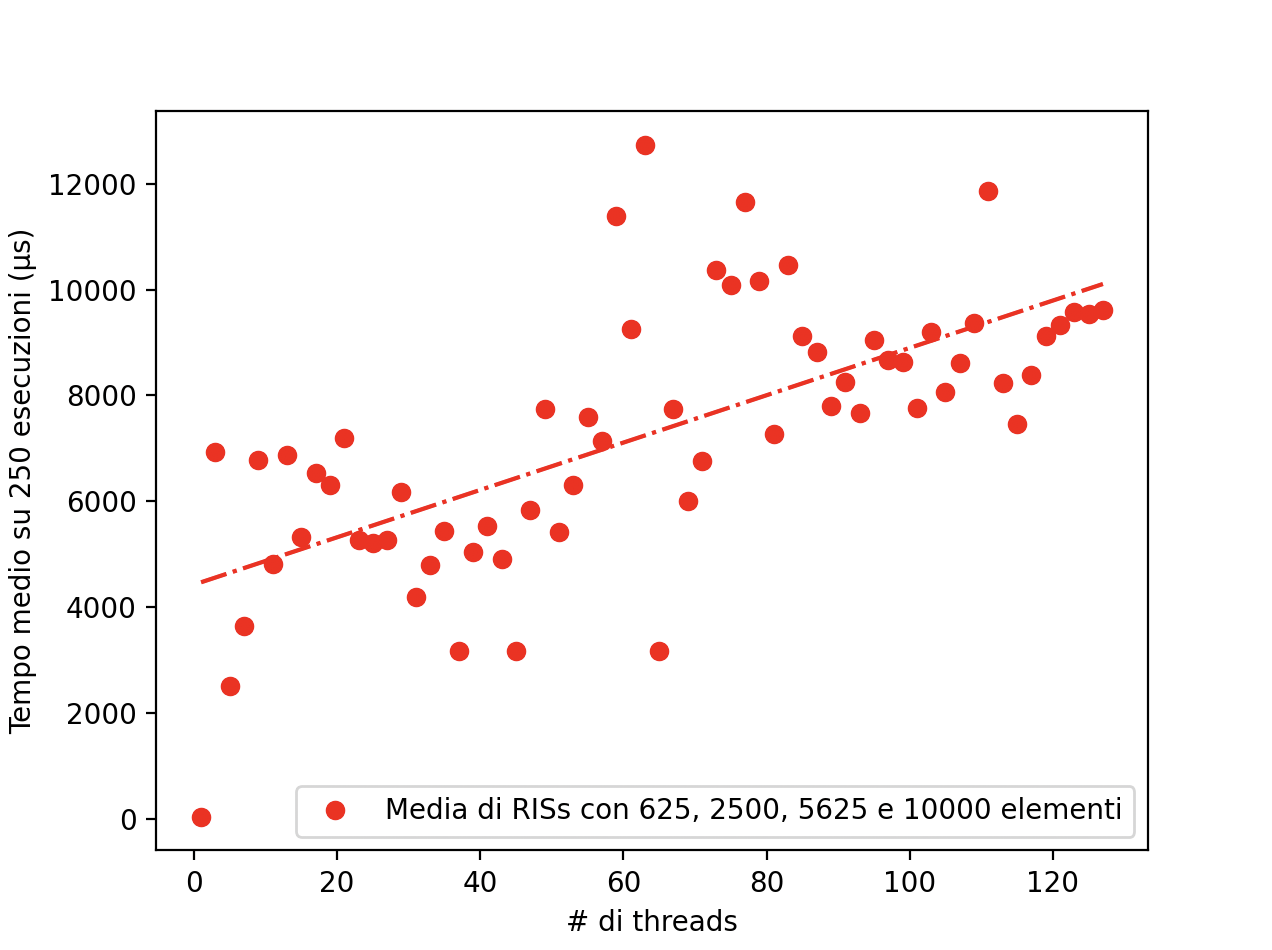
\includegraphics[width=.6\textwidth]{images/results/gain-serial-time.png}
  \caption{Delta del tempo di esecuzione tra la fine dell'ultimo thread e la
  fine della procedura \texttt{gain\_compute\_phase}}
  \label{fig:serial-time}
\end{figure}

Si vuole portare l'attenzione sulle righe 37-41: in questo \texttt{for} si effettua
l'attesa, tramite la funzione \texttt{pthread\_join}, e la somma dei risultati
parziali di ogni thread nella matrice \texttt{phase}. Anche se la procedura
\texttt{gsl\_matrix\_complex\_add} potrebbe sembrare un rallentamento, in realtà,
tramite il \textit{pipelining} delle operazioni di creazione dei thread, questo costo
è ammortizzato e non influisce significativamente sul tempo di esecuzione. In
figura \ref{fig:gain-compute-phase-pipeline} è possibile osservare una
rappresentazione grafica di questo processo tramite un esempio con 4 thread: l'obiettivo
è quello di assicurarsi che la procedura tra $t_{4}$ e $t_{5}$ sia la più breve possibile,
in modo da non rallentare l'intero processo. In figura \ref{fig:serial-time} è possibile
osservare le misurazioni di $t_{5}- t_{4}$, che risulta essere con un trend
crescente, ma comunque contenuto.

\begin{figure}
  \centering
  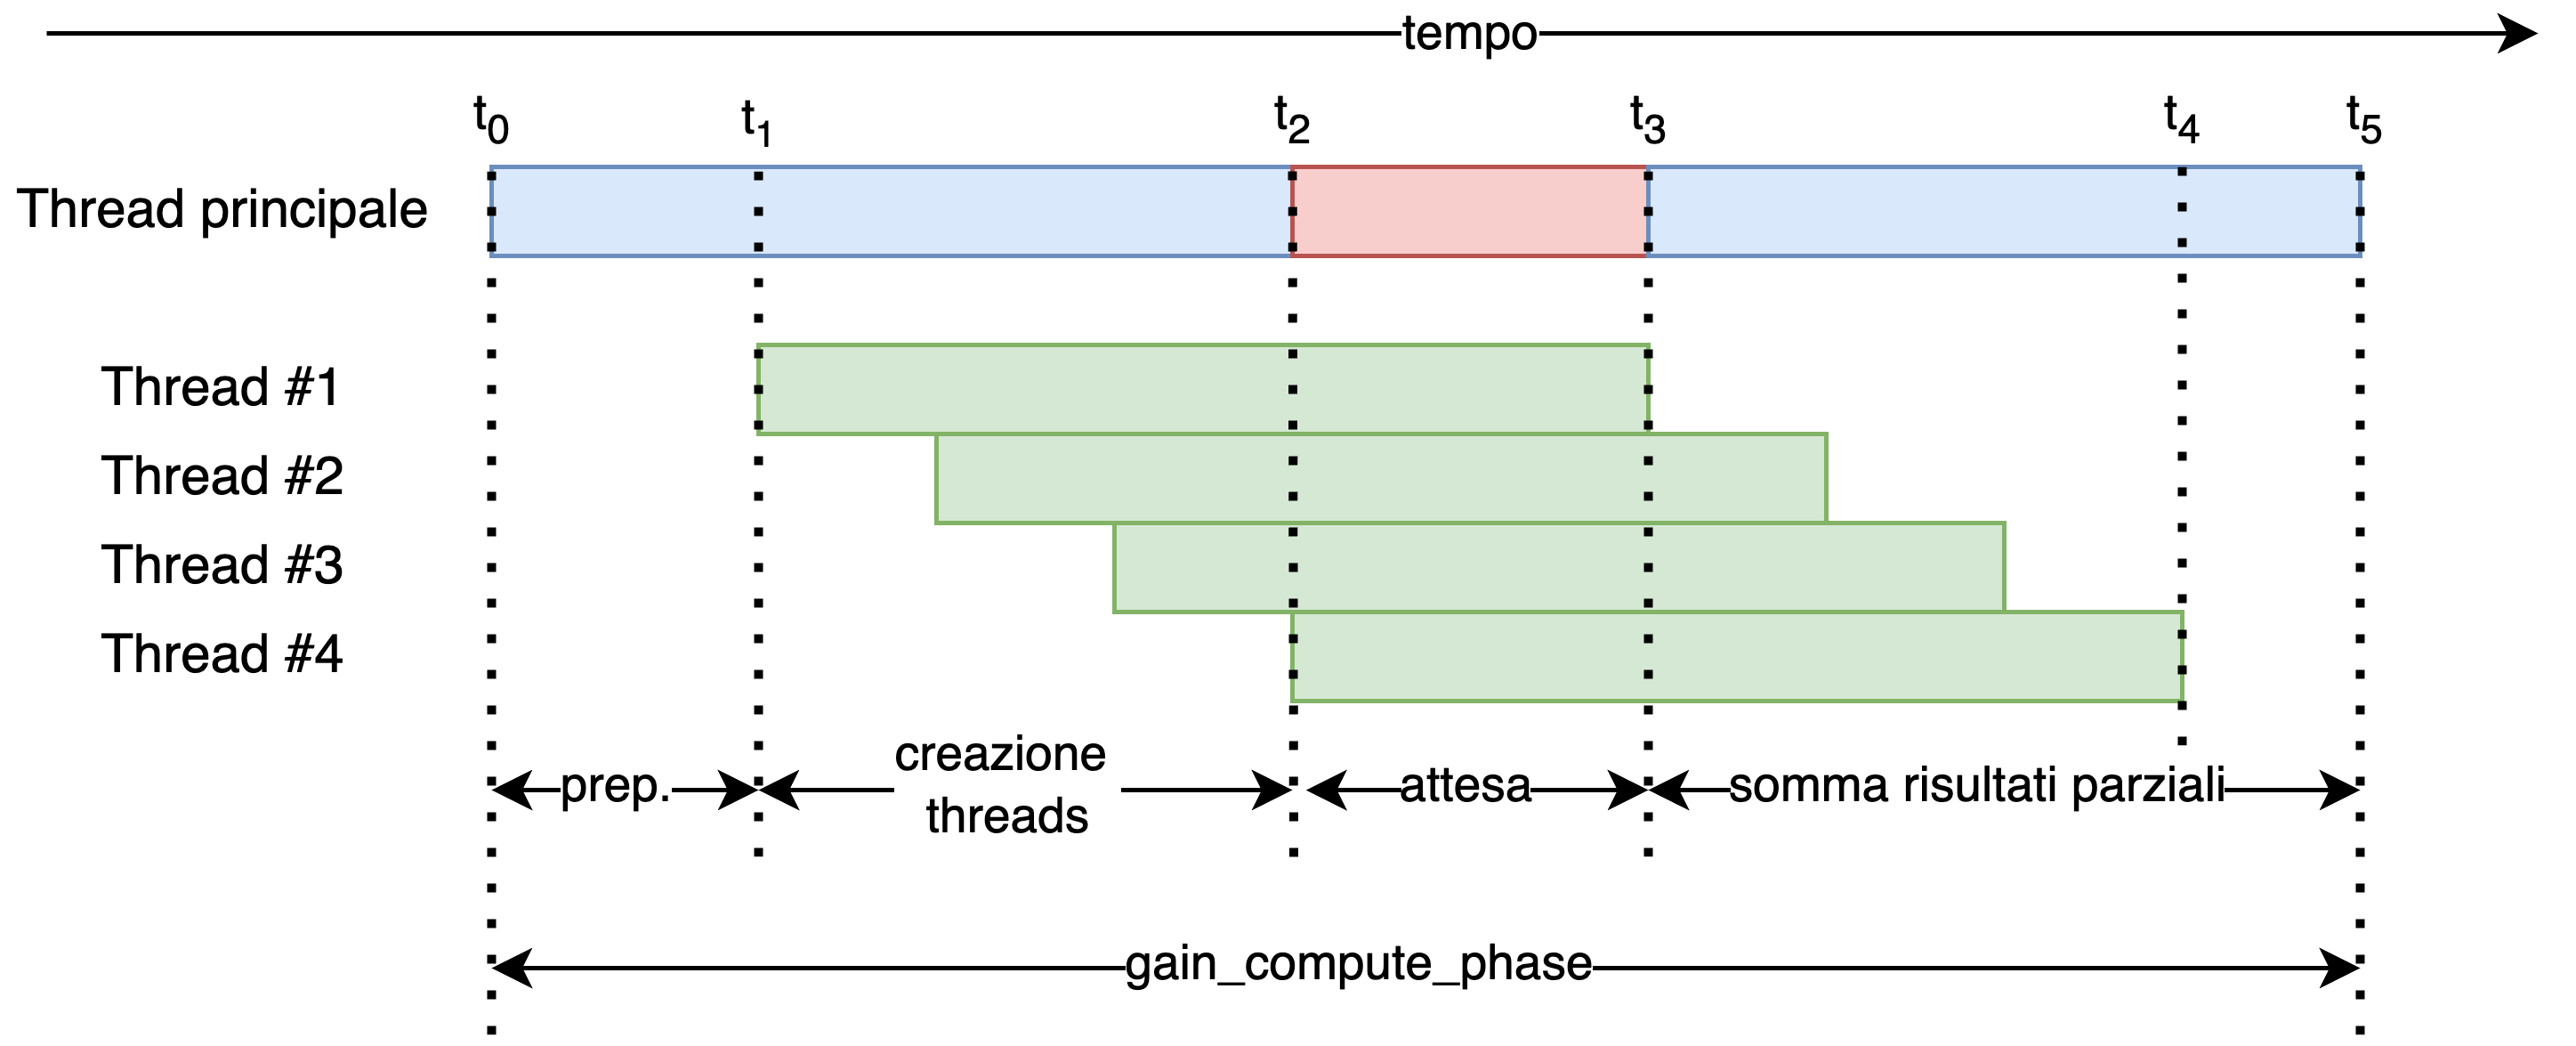
\includegraphics[width=\textwidth]{
    images/examples/gain_compute_phase-pipeline.png
  }
  \caption{Rappresentazione grafica della sequenza temporale delle operazioni
  eseguite da \texttt{gain\_compute\_phase}}
  \label{fig:gain-compute-phase-pipeline}
\end{figure}

\subsection{Parallelizzazione su GPU}
\label{subsec:cuda}

Come anticipato nel capitolo \ref{sec:contributo}, le implementazioni tramite
GPU sono state realizzate utilizzando le librerie \textit{CUDA}\cite{cuda} e
\textit{OpenCL}\cite{opencl}. La prima è una libreria sviluppata da \textit{NVIDIA}
e supporta solo le GPU di questo produttore, mentre la seconda è una libreria cross-platform
sviluppata da \textit{Khronos Group} e supporta praticamente tutte le
piattaforme disponibili. La programmazione su GPU è un approccio molto differente
rispetto al \textit{multi-threading}, data la completa differenza di architettura
rispetto le CPU. In aggiunta le due librerie presentano delle differenze
sostanziali che ne influenzano di molto l'implementazione, ma possiedono anche degli
aspetti che le accomunano. Entrambe permettono di sfruttare l'architettura
\textit{SIMT} discussa nel paragrafo \ref{para:simt}. Esse prevedono funzioni
denominate \textit{kernel}, ovvero le procedure definite per essere eseguite sul
\textit{device} (GPU), le quali sono invocate dall'\textit{host} (CPU). La
principale differenza tra le due è che \textit{CUDA} genera il codice \textit{kernel}
in fase di compilazione tramite il predisposto compilatore \texttt{nvcc}, mentre
OpenCL genera il codice \textit{device} in fase di esecuzione poiché, essendo
una libreria cross-platform, non può conoscere a priori il dispositivo di destinazione.
Queste divergenze comportano che a parità di complessità del codice, \textit{CUDA}
risulti più performante in quanto maggiormente ottimizzata rispetto allo
specifico target, mentre \textit{OpenCL} rimane più flessibile e portabile\cite{cudavsopencl}.

Il primo passo per la realizzazione è stato quello di identificare come integrare
il codice della libreria \textit{CoopeRIS} con le librerie di programmazione su
GPU. L'approccio scelto è stato quello di mantenere il codice della procedura \texttt{gain}
invariato e di sostituire il calcolo della matrice \texttt{phase} tramite un \textit{kernel}
creato ad hoc.

\paragraph{Implementazione tramite \textit{CUDA}}
\label{para:cuda}

Nel listato \ref{lst:cuda-kernel} è possibile osservare il codice del \textit{kernel}
definito secondo la sintassi \textit{CUDA} per il calcolo della matrice \texttt{phase}
per singolo elemento della RIS in posizione $n, m$. Per ottimizzare al massimo
le prestazioni la procedura originaria (righe 21-42 del listato \ref{lst:gain})
è stata semplificata algebricamente.

\vspace{1em}
\lstinputlisting[caption=\textit{Kernel} \textit{CUDA} per il calcolo di \texttt{phase},
language=C++, label=lst:cuda-kernel]{listings/cuda-kernel.cpp}
\vspace{1em}

Di seguito si trova una breve descrizione della procedura:

\begin{itemize}
  \item Nella prima riga si definisce la firma del \textit{kernel}, con i parametri
    necessari per effettuare la computazione. Le variabili \texttt{k\_du\_sin\_cos},
    \texttt{k\_du\_sin\_sin}, \texttt{phase\_real} e \texttt{phase\_imag} sono
    puntatori alla memoria globale del \textit{device}, \texttt{n} e \texttt{m}
    sono gli indici dell'elemento della RIS in fase di calcolo, \texttt{PHI} e
    \texttt{alpha} rappresentano rispettivamente lo sfasamento della segnale secondo
    l'attuale configurazione della RIS e lo sfasamento dovuto alla posizione dovuta
    al trasmettitore, ed infine \texttt{size} è la dimensione della matrice linearizzata
    \texttt{phase};

  \item Riga 2 rappresenta il principio fondamentale della programmazione tramite
    la tecnica \textit{SIMT}: ogni thread riceve qui dal proprio contesto l'indice
    $i$ dell'elemento della matrice \texttt{phase} su cui dovrà lavorare. La ragione
    per cui è necessario ricavarlo dalla moltiplicazione di \texttt{blockIdx.x}
    per \texttt{blockDim.x} e \texttt{threadIdx.x} è indicata nei paragrafi
    successivi;

  \item Per spiegare lo scopo dell'\texttt{if} a riga 3, si deve fare riferimento
    al funzionamento della tecnica \textit{SIMT}: la creazione dei thread avviene
    a blocchi di thread, la cui grandezza non è necessariamente un multiplo
    della dimensione della matrice \texttt{phase}. Per evitare che thread non
    necessari eseguano operazioni inutili su memoria non allocata, è necessario controllare
    che l'indice \texttt{i} sia minore del numero di elementi della RIS;

  \item A riga 4 è computato il valore della componente che in equazione \ref{eq:power}
    è espressa da $-j(\Phi_{m,n}+\Theta_{m,n})$. Dato che $\Phi_{m,n}$ e
    $\Theta_{m,n}$ appartengono a $\mathbb{R}$, in questo calcolo non è necessario
    memorizzare la parte reale dal momento che essa sarà sempre pari a zero;

  \item Le righe 5-6 infine implementano l'esponenziazione del precedente valore
    calcolato, come in equazione \ref{eq:power}, tramite l'applicazione dell'equazione
    di Eulero.
\end{itemize}

L'effettiva integrazione di questa procedura nel codice della libreria \textit{CoopeRIS}
è stata realizzata tramite la creazione di funzioni di supporto per l'inizializzazione,
l'allocazione, deallocazione e copia della memoria sul \textit{device} e l'invocazione
del \textit{kernel}. Nel listato \ref{lst:cuda-gain} è possibile osservare la
corrispettiva funzione di calcolo della matrice \texttt{phase} tramite \textit{CUDA}.

\vspace{1em}
\lstinputlisting[caption=Funzione del calcolo di \texttt{phase} tramite \textit{CUDA},
language=C++, label=lst:cuda-gain]{listings/cuda-gain.cpp}
\vspace{1em}

Come si può notare, questa procedura è molto simile rispetto quella originaria: la
principale differenza risiede nelle allocazioni e copia della memoria dall'\textit{host}
al \textit{device} e viceversa, e nell'invocazione di una funzione \textit{wrapper}
che è responsabile dell'invocazione del \textit{kernel}, osservabile nel listato
\ref{lst:cuda-kernel-wrap}.

\vspace{1em}
\lstinputlisting[caption=Funzione \textit{wrapper} per l'invocazione del \textit{kernel}
\textit{CUDA}, language=C++, label=lst:cuda-kernel-wrap]{listings/cuda-kernel-wrap.cpp}
\vspace{1em}

In questa procedura si può notare la principale caratteristica della sintassi
\textit{CUDA}: all'interno delle parentesi angolari \texttt{<<<num\_blocks, max\_threads\_per\_block
>>>} si specificano rispettivamente il numero di blocchi e la quantità di thread
invocati per blocco. Questi valori definiscono l'\textit{occupancy} del \textit{kernel},
ovvero il rapporto tra il numero di thread attivi e il numero massimo di thread per
blocco. Più alto è questo valore, più efficiente è l'utilizzo della GPU. Un
blocco è un insieme di thread che condividono la stessa memoria locale e possono
sincronizzarsi tra di loro, mentre un insieme di blocchi di thread è definito \textit{grid}.
Il numero di blocchi è determinato dal rapporto dalla grandezza del problema per
il numero di thread per blocco, mentre quest'ultimo è un parametro arbitrario la
cui scelta fa parte di un processo iterativo che richiede esperienza e test
approfonditi, ma è possibile ottenere un buon compromesso considerando i seguenti
fattori:

\begin{itemize}
  \item È generalmente consigliabile di utilizzare un numero di thread per blocco
    multiplo della dimensione del \textit{warp}, ovvero il numero di thread che in
    \textit{SIMT} è eseguito in maniera sincrona, il quale nelle architetture \textit{CUDA}
    è pari a 32;

  \item Il suo valore massimo è definito dall'architettura fisica della GPU,
    ottenibile tramite delle apposite interrogazioni alle API di \textit{CUDA};

  \item Se il \textit{kernel} è computazionalmente molto pesante e richiede
    molta memoria condivisa, è consigliabile ridurre il numero di thread per blocco
    per evitare di saturarla;
\end{itemize}

Questa è la ragione per la quale l'indice \texttt{i}, ottenuto nel listato
\ref{lst:cuda-kernel}, si è dovuto calcolare come \texttt{i = blockIdx.x *
blockDim.x + threadIdx.x}, infatti \texttt{blockIdx.x} rappresenta l'indice del
blocco corrente, \texttt{blockDim.x} il numero di thread per blocco e \texttt{threadIdx.x}
l'indice del thread all'interno del blocco.

\paragraph{Implementazione tramite \textit{OpenCL}}
\label{para:opencl}

Ciò che differenzia maggiormente l'implementazione tramite \textit{OpenCL}
rispetto \textit{CUDA} è la necessità di compilare la funzione \textit{kernel}
in fase di esecuzione. Questo comporta che questa soluzione richieda una ulteriore
configurazione in fase di creazione dell'istanza RIS per rispettare i vincoli sopracitati.
Per permettere ad un utente con molteplici piattaforme supportate da \textit{OpenCL},
sono stati introdotti due nuovi parametri nella configurazione dell'ambiente di
simulazione \textit{OMNeT++}: \texttt{openclPlatformId} e \texttt{openclDeviceId},
che consentono rispettivamente di selezionare la piattaforma e il dispositivo su
cui esso desidera eseguire il calcolo. Per il resto, il funzionamento della procedura
\textit{kernel} e delle invocazioni alle API di \textit{OpenCL} sono concettualmente
identiche a quelle di \textit{CUDA} e per questa ragione omesse in questa
sezione.

\section{Discussione e Valutazione}
\label{ch:discussione}

In questo capitolo si vuole portare un analisi qualitativa delle soluzioni proposte
per l'ottimizzazione della libreria \textit{CoopeRIS}. Si discuteranno i vantaggi
e gli svantaggi di ciascuna soluzione, i limiti e le sfide affrontate durante lo
sviluppo, e si valuterà l'efficacia delle stesse rispetto l'obiettivo prefissato.

\subsection{Vantaggi delle soluzioni implementate}
\label{subsec:vantaggi}

Molti sono i vantaggi che le soluzioni proposte apportano alla libreria \textit{CoopeRIS}.
I principali sono la riduzione del tempo di esecuzione, il supporto multi-piattaforma
e la possibilità di sfruttare hardware dedicato. Questi aspetti sono considerati
come le principali esigenze che hanno portato alla scelta di intraprendere
questo progetto.

\paragraph{Performance e tempo di esecuzione}
\label{para:performance}

Il primo e più importante beneficio del calcolo parallelo è la riduzione del
tempo di esecuzione. Questo è stato confermato dai risultati ottenuti durante le
fasi di \textit{benchmarking} della libreria stessa oltreché nel framework di
simulazione completo, discussi nel dettaglio nel capitolo \ref{ch:risultati}. Il
risparmio di tempo di esecuzione è il motivo principale per cui si è scelto di
intraprendere questo progetto, e tutte e tre le implementazioni hanno dimostrato
di essere efficaci secondo questo criterio. La soluzione mediante \textit{CUDA} ha
dimostrato di essere la più performante, seguita da quella tramite \textit{OpenCL}
e infine \textit{multi-threading}. Questo risultato è in linea con le aspettative,
e per questo motivo il progetto è stato considerato come un discreto successo.

\paragraph{Supporto multi-piattaforma}
\label{para:supporto}

Un ulteriore vantaggio significativo, soprattutto in riferimento all'adozione di
\textit{OpenCL} come soluzione, risiede nella capacità di impiegare la libreria su
una vasta gamma di piattaforme diverse. Tale caratteristica rappresenta un
elemento di primaria importanza per garantire la massima compatibilità e
portabilità del codice, consentendo di svincolare l'utente dal fenomeno del \textit{vendor
lock-in}. Questo problema è frequentemente riscontrato nell'utilizzo di soluzioni
proprietarie come \textit{CUDA}. La possibilità di mantenere l'indipendenza dal fornitore
specifico di hardware o software conferisce un valore aggiunto notevole,
promuovendo un ecosistema di sviluppo più aperto e flessibile.

\subsection{Svantaggi delle soluzioni implementate}
\label{sec:svantaggi}

Nonostante i vantaggi, le soluzioni proposte presentano anche degli svantaggi
che ne limitano l'utilizzo e l'efficacia. Principalmente, si possono
identificare la leggibilità e manutenibilità del codice e la richiesta di
hardware dedicato. Importante è anche considerare che le soluzioni proposte non sono
state progettate per essere utilizzate in maniera combinata, ma piuttosto come
alternative tra cui l'utente può scegliere in base alle proprie esigenze, e per questo
motivo il beneficio rispetto lo sforzo richiesto è limitato.

\paragraph{Leggibilità e manutenibilità del codice}
\label{para:leggibilita}

Un aspetto negativo di questo progetto è la complessità aggiunta al codice della
libreria \textit{CoopeRIS}, soprattutto derivante dalla necessità di mantenere tre
diverse implementazioni per la stessa funzionalità, scritte secondo tre diversi
paradigmi e convenzioni. Questo rende di molto più difficile la comprensione del
codice, specialmente per utenti non confidenti con la programmazione parallela o
i framework di calcolo su GPU. Questo rappresenta un ostacolo non indifferente,
soprattutto nell'ottica di futuri sviluppi.

\paragraph{Richiesta di hardware dedicato}
\label{para:hardware}

Un ulteriore critica nei confronti di questo progetto è la necessità di hardware
specifico e dedicato per poter sfruttare le implementazioni ottimizzate, soprattutto
per quanto riguarda le soluzioni tramite \textit{CUDA} e \textit{OpenCL}. Questa
è stata la principale motivazione che ha portato alla scelta di adoperare anche
una implementazione \textit{multi-threading}, poiché è l'unica tra le tre che
non richiede hardware aggiuntivo.

\subsection{Limiti e sfide affrontate}
\label{subsec:limiti}

Le principali sfide affrontate durante lo sviluppo di questo progetto sono state
la complessità del codice e la necessità di costruire un'architettura modulare che
permettesse di mantenere le tre diverse implementazioni in maniera ordinata.
Questo ha richiesto una meticolosa progettazione e un'attenta implementazione, che
ha richiesto molto tempo e sforzo. Un altro ostacolo è stato la necessità di
apprendere nuove tecnologie e paradigmi di programmazione, come la programmazione
su GPU, che ha richiesto un periodo di studio e apprendimento prima di poter
essere implementata correttamente. Infine, l'ultimo aspetto critico è stato la
necessità di effettuare dei test approfonditi e di profilare il codice per
garantire la correttezza di tutte e tre le implementazione e che esse fossero
effettivamente più performanti rispetto la soluzione originaria.